\typeout{NT FILE chapter6.tex}
\chapter{Final model and evaluation}
\section{Final Model}
\paragraph{}
The best model found was that from the hyperparameter tuning performed on the new \textit{JP2} data in Section \ref{hp_new_data}, the performance of this model was summarised in Table \ref{tab_hp}, which shows a Dice Score on the test dataset of $95\%$. More in-depth analysis per epoch will now be performed in this section.
\paragraph{}
As it can be seen from Figure \ref{best_loss}, there is no evidence of overfitting before the Early Stopping strategy kicks off at the 88th epoch. It can also be seen from Figure \ref{best_dice}, that the Training and Validation curve follow a similar shape with less fluctuation towards the final epochs, as would be expected from a well-performing model.

\begin{figure}[hbt!]
    % \centering
    \begin{minipage}[c]{0.5\linewidth}
    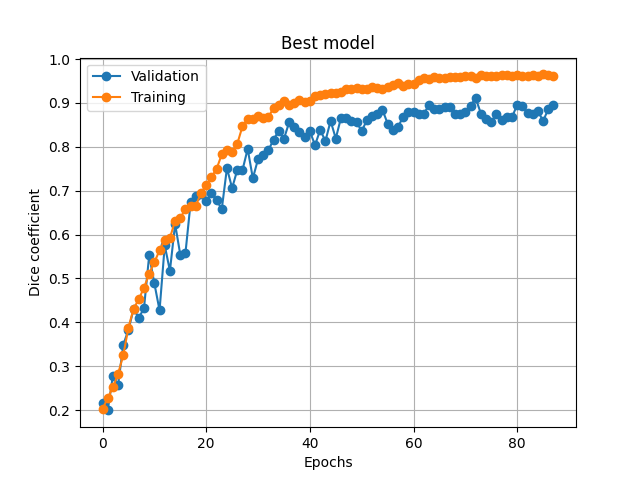
\includegraphics[width=\linewidth]{Best model_Dice coefficient.png}
    \caption{Dice Score comparison}
    \label{best_dice}
    \end{minipage}
        \hfill
        \begin{minipage}[c]{0.5\linewidth}
        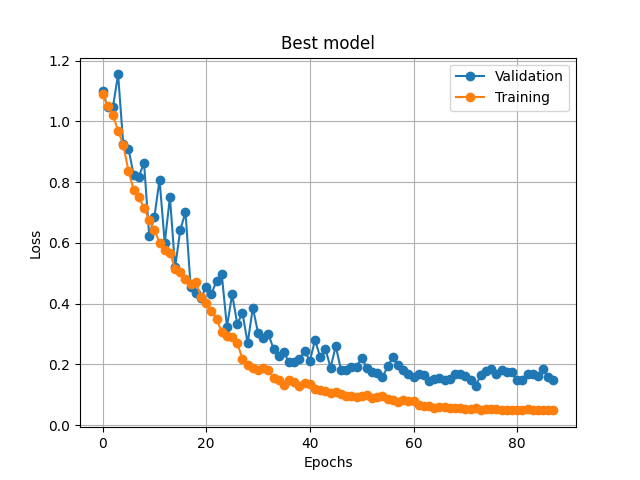
\includegraphics[width=\linewidth]{Best model_Loss.png}
        \caption{Loss
        comparison}
        \label{best_loss}
    \end{minipage}
\end{figure}


% \begin{figure}[hbt!]
%     \centering
%     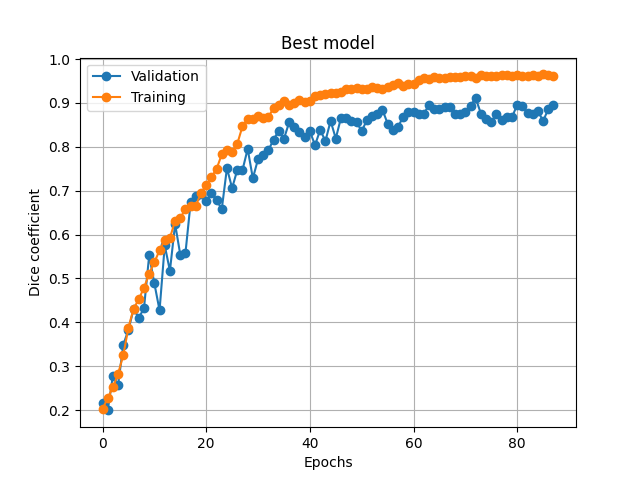
\includegraphics[width=1 \textwidth]{Best model_Dice coefficient.png}
%     \caption{Best Model Training and Validation Dice Score comparison)}
%     \label{fig_tp_fp}
% \end{figure}

% \begin{figure}[hbt!]
%     \centering
%     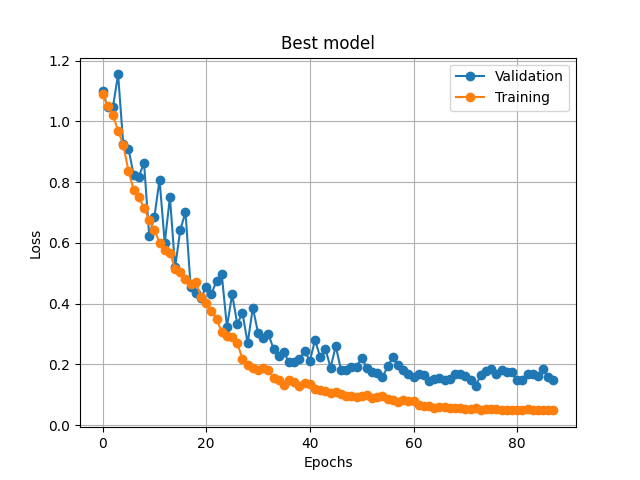
\includegraphics[width=1 \textwidth]{Best model_Loss.png}
%     \caption{Best Model Training and Validation Loss
%      comparison)}
%     \label{fig_tp_fp}
% \end{figure}
% \begin{figure}[hbt!]
%     \centering
%     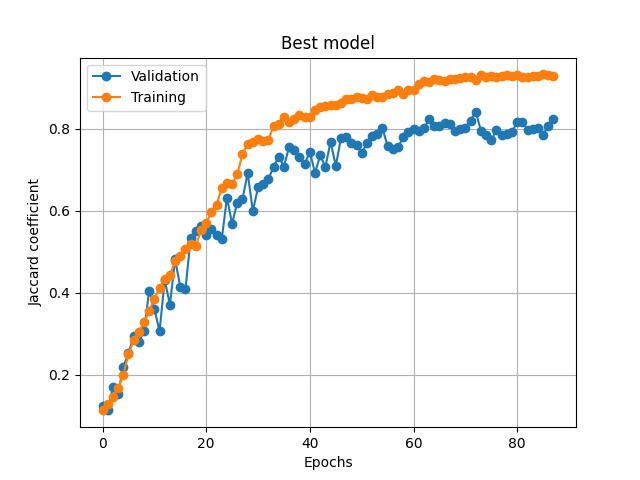
\includegraphics[width=1 \textwidth]{Best model_Jaccard coefficient.png}
%     \caption{Best Model Training and Validation Jaccard Score comparison)}
%     \label{fig_tp_fp}
% \end{figure}

\section{Test Evaluation}

During the Training/ Validation/ Test split process $39$ images were assigned to the test set, that is completely unseen data by the model. Using the best model's frozen weights (the best weights are restored as part of the Early Stopping strategy) and architecture, inference is performed of the test dataset to assess model performance by comparing the predictions against the ground truth mask.

\paragraph{}
The overall performance of the model at image level is summarised in Table \ref{sum_test}, where $3$ categories are defined according to model performance, the individual performance evaluation scores of each test image are then compared in Figure \ref{scatter_test_scores} according to those categories.

    \begin{table}[ht!] 
        \begin{center}
        \begin{tabular}{ccc} 
        \toprule
        \textbf{Category} & \textbf{Dice Score range}  & \textbf{Number of images}  \\ \midrule
        High & Greater than or equal to 0.7 & 29  \\
        Medium & Between 0.7 and 0.4 & 5  \\
        Low & Smaller or equal to 0.4 & 5  \\
    \bottomrule
        \end{tabular}
      \end{center} 
      \caption{Dice score test image summary}\label{sum_test}
    \end{table}
    \begin{figure}[hbt!]
        \centering
        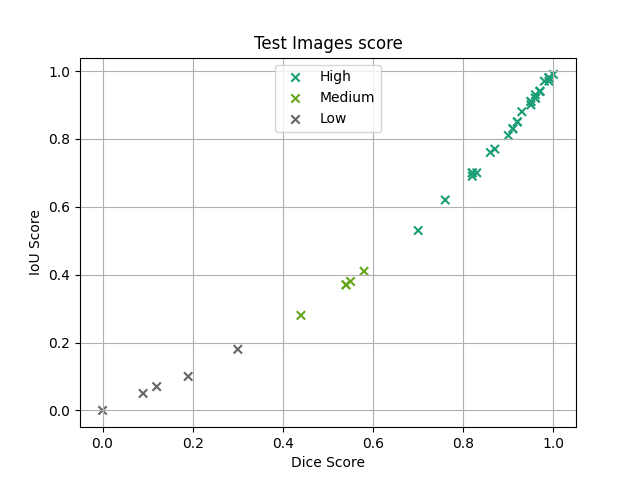
\includegraphics[width=0.75 \textwidth]{test images scores.png}
        \caption{Dice Score vs. \gls{IoU} Score Test images scatter plot}
        \label{scatter_test_scores}
    \end{figure}
\paragraph{}
A short image by image analysis will be performed for $2$ images of each category, where purple colour represents background (non-\gls{RTS}) pixels and yellow represents foreground (\gls{RTS}) pixels, with varying opacity according to prediction confidence, the lighter the shade the lower the confidence, there is also a red contour which represents the ground truth mask outline.
\paragraph{}
As can be seen from Figure \ref{high_score_pic} the algorithm can deal with both simpler thaw slump shapes (on the left) and more complex shapes (on the right), although the latter shows lower confidence in the pixel prediction confidence, as can be seen by lower intensity pixel shading and is also reflected in a lower dice score.

    \begin{figure}[hbt!]
        % \centering
        \begin{minipage}[c]{0.55\linewidth}
        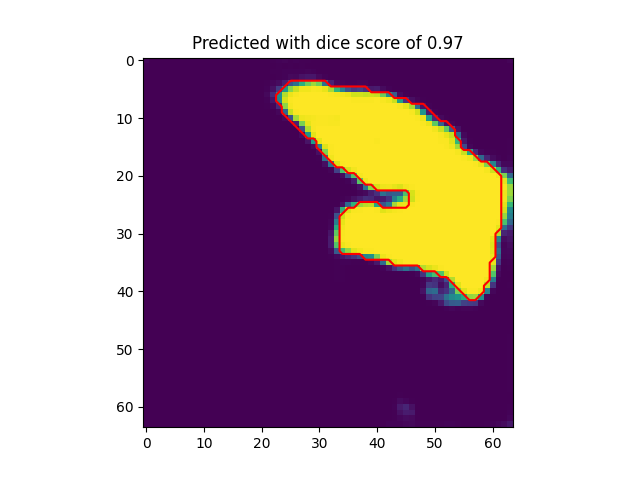
\includegraphics[width=\linewidth]{1_0.97.png}
        \label{best_dice}
        \end{minipage}
            \hfill
            \begin{minipage}[c]{0.55\linewidth}
            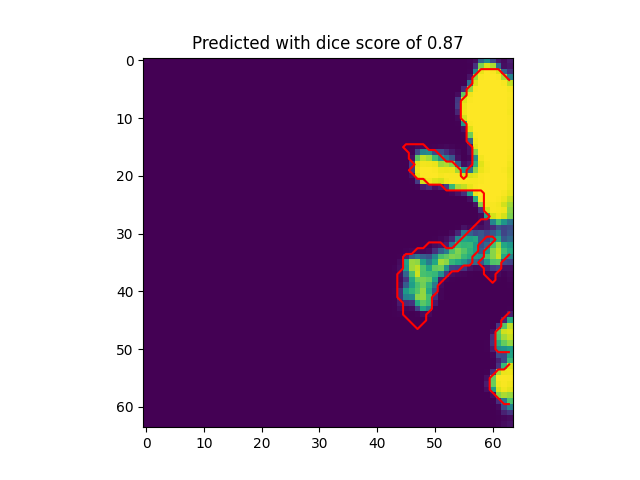
\includegraphics[width=\linewidth]{25_0.87.png}
            \label{high_score_pic}
        \end{minipage}
        \caption{Test set predicted vs. ground truth high score examples}
    \end{figure}

The model struggles with elongated thaw slumps as seen in Figure \ref{medium_score_pic} on the left and in some instances correctly predicts the thaw slump \gls{ROI} but also predicts False Positive \gls{RTS} which then has an impact on the dice score (right side). This presence of False Positives could be an indication of an actual \gls{RTS}, which has not been labeled yet. Due to the lack of expert knowledge, these False Positives have not been validated but could point researchers in the right direction when looking for new \gls{RTS}.

    \begin{figure}[hbt!]
        % \centering
        \begin{minipage}[c]{0.55\linewidth}
        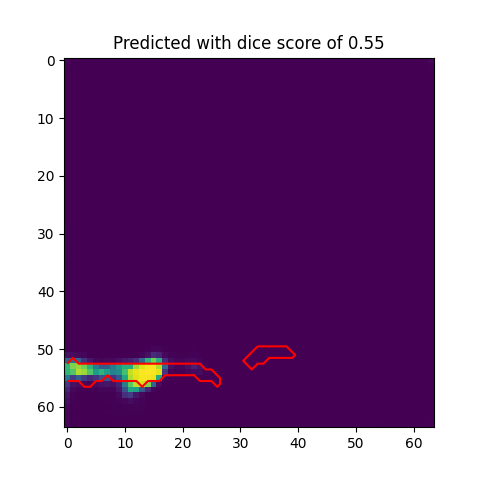
\includegraphics[width=\linewidth]{11_0.55.png}
        \label{best_dice}
        \end{minipage}
            \hfill
            \begin{minipage}[c]{0.55\linewidth}
            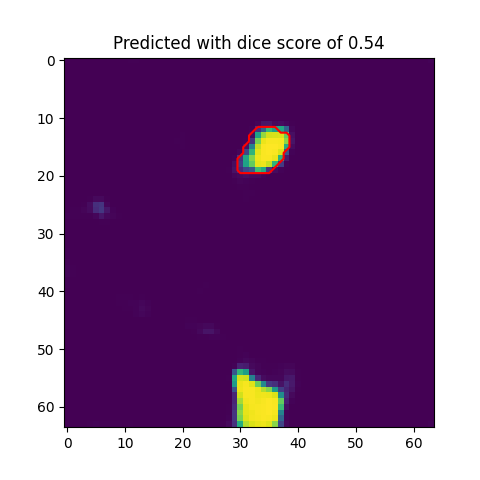
\includegraphics[width=\linewidth]{10_0.54.png}
            \label{medium_score_pic}
        \end{minipage}
        \caption{Test set predicted vs. ground truth medium score examples}
    \end{figure}

 The really low performing test images can be seen in Figure \ref{low_score_pic}, the model seems to not be very good at predicting very small \gls{RTS}, this could be due to the fact that each pixel represents a \SI{10}{\metre\squared} area and some \gls{RTS} may be smaller than that, or that the image reprojection has a slight misalignment, as can be seen from the image on the left which predicts a False Positive \gls{RTS} to the left of the ground truth red contour.

    \begin{figure}[hbt!]
        % \centering
        \begin{minipage}[c]{0.55\linewidth}
        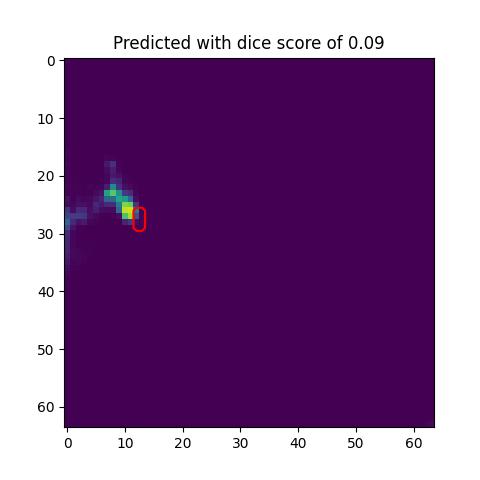
\includegraphics[width=\linewidth]{19_0.09.png}
        \label{best_dice}
        \end{minipage}
            \hfill
            \begin{minipage}[c]{0.55\linewidth}
            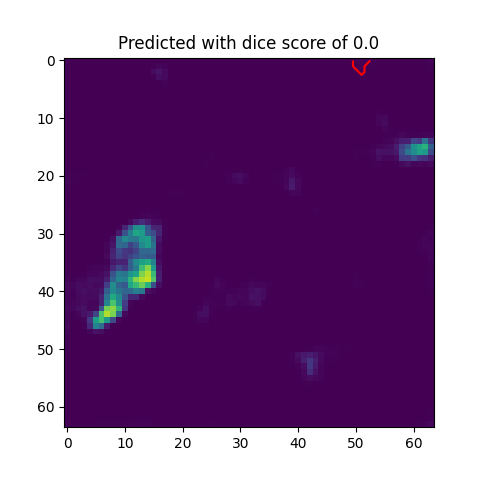
\includegraphics[width=\linewidth]{31_0.0.png}
            \label{low_score_pic}
        \end{minipage}
        \caption{Test set predicted vs. ground truth low score examples}
    \end{figure}

Another level of analysis involves looking at the input images (X) next to the ground truth and predictions (y and predicted y) to check if there is any visible evidence of the assumptions made above. An example of this can be seen in Figure \ref{medium_score_input_pic}. By analysing the input image (on the left), it can be seen that the image is corrupted at the top. This could be perhaps due to an error in the multispectral instrument during the collection, or perhaps during further post-processing. When it comes to the \gls{RTS} \gls{ROI}, the lighter shading in the input image corresponds to the predicted area on the right side, indicating that perhaps the reprojection of the labelled data (red contour) to the input image's \gls{CRS} is incorrect and the algorithm is indeed more accurate than the dice score of $58\%$ seems to suggest.
    % \begin{figure}[hbt!]
    %     \centering
    %     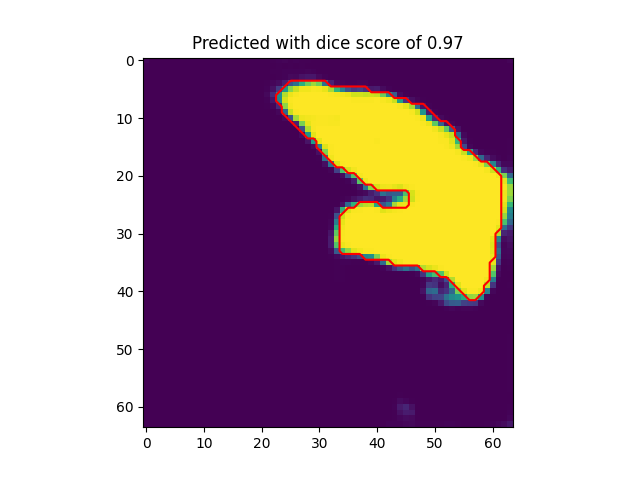
\includegraphics[width= \textwidth]{1_0.97.png}
    %     \caption{Test set predicted vs. ground truth high score example}
    %     \label{fig_tp_fp}
    % \end{figure}
    \begin{figure}[hbt!]
        \centering
        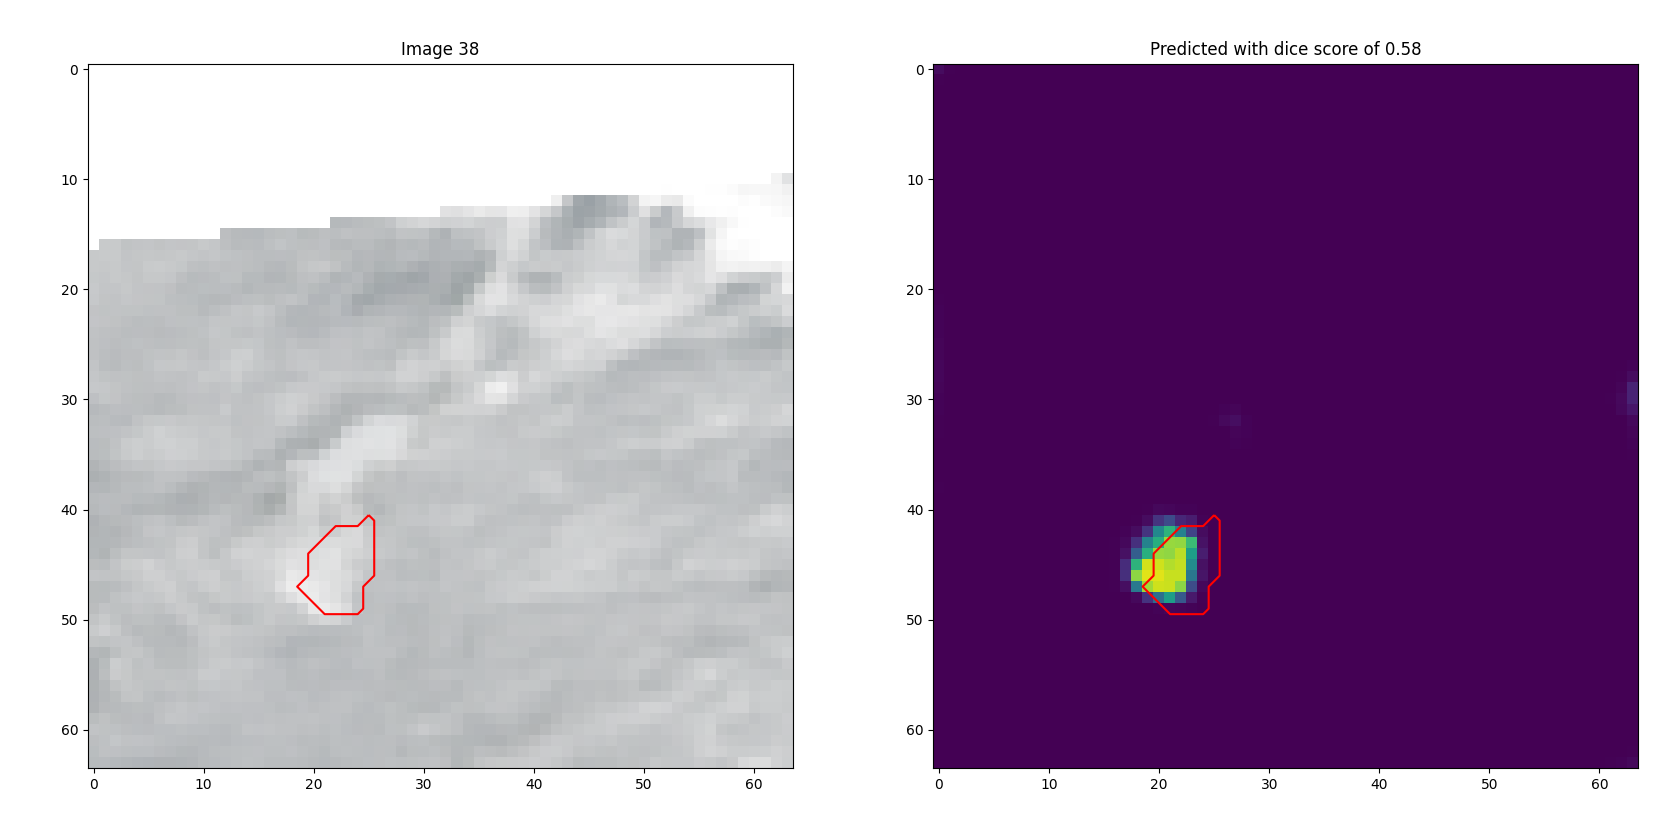
\includegraphics[width=1\textwidth]{38_0.58_input.png}
        \caption{Test set predicted vs. ground medium score example}
        \label{medium_score_input_pic}
    \end{figure}
    % \begin{figure}[hbt!]
    %     \centering
    %     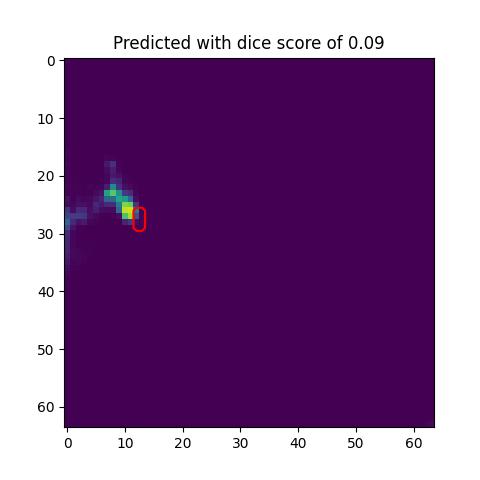
\includegraphics[width=0.75 \textwidth]{19_0.09.png}
    %     \caption{Test set predicted vs. ground truth low score example}
    %     \label{low_score_pic}
    % \end{figure}

Given more time, all the above assumptions would be investigated further.